
\documentclass[12pt]{article}

\usepackage{graphicx}
%\usepackage{subcaption}
\usepackage{amsmath}
\usepackage{amssymb}
%\usepackage{afterpage}
%\usepackage{showlabels}
% \usepackage{epstopdf}
% \usepackage{pdfpages}
\usepackage{geometry}
%\usepackage{wrapfig}
\usepackage{url}
\usepackage{times}
\usepackage{pdfpages}
\usepackage{etoolbox}
\usepackage{hyperref}
\hypersetup{
    colorlinks=true,
    linkcolor=blue,
    filecolor=magenta,
    urlcolor=cyan,
    pdftitle={Overleaf Example},
    pdfpagemode=FullScreen,
    }

\urlstyle{same}

%\usepackage{cprog}
%\usepackage[compact]{titlesec}
%\titlespacing{\section}{0pt}{5pt}{5pt}
%\titlespacing{\subsection}{0pt}{*0}{*0}
%\titlespacing{\subsubsection}{0pt}{*0}{*0}
%\usepackage[belowskip=-10pt,aboveskip=0pt,margin=10pt,font=footnotesize,labelfont=bf]{caption}

\newcommand{\shortlist}{%
\parindent 0in%
\parskip   0in%
\itemsep   0in%
\topsep    0in%
\parsep    0in%
}

% \setlength{\parskip}{0pt}
% \setlength{\parsep}{0pt}
% \setlength{\headsep}{0pt}
% \setlength{\topskip}{0pt}
% \setlength{\topmargin}{0pt}
% \setlength{\topsep}{0pt}
% \setlength{\columnsep}{0pt}
%\linespread{0.95}

% cost status:
% available: 193,022.87
% liwei (3.5 months): 13555
% me (2 months): 13653
% fringe (13555*.45 + 13653*.079) = 7178
% steve (2 months): 7155
% shujie (2 months): 6700
% total direct: 48241
% total (*1.47): 70914
% available 7/15: 122109

\setlength{\parindent}{0in}

\geometry{letterpaper,tmargin=1in,bmargin=1in,lmargin=1in,rmargin=1in}

%\renewcommand{\normalsize}{\fontsize{11pt}{13.2pt}\selectfont}\normalsize

% \renewcommand{\topfraction}{0.9}	% max fraction of floats at top
% \renewcommand{\bottomfraction}{0.8}	% max fraction of floats at bottom
% % Parameters for TEXT pages (not float pages):
% \setcounter{topnumber}{2}
% \setcounter{bottomnumber}{2}
% \setcounter{totalnumber}{4}     % 2 may work better
% \setcounter{dbltopnumber}{2}    % for 2-column pages
% \renewcommand{\dbltopfraction}{0.9}	% fit big float above 2-col. text
% \renewcommand{\textfraction}{0.07}	% allow minimal text w. figs
% % Parameters for FLOAT pages (not text pages):
% \renewcommand{\floatpagefraction}{0.7}	% require fuller float pages
% % N.B.: floatpagefraction UST be less than topfraction !!
% \renewcommand{\dblfloatpagefraction}{0.7}	% require fuller float pages


%\renewcommand{\familydefault}{\sfdefault}

% TODO
% add figures
% too much?
% look at links (incl comp)
% href
% what to do about points / free choice?

\newcommand{\Title}{PHYS 615 -- HW 2}

\begin{document}

\begin{center}
{\Large\bfseries\Title}

\end{center}
\bigskip
\bigskip

% \begin{tabular}{p{1.7in}p{4in}}
% DOE award number: & DE-SC0006670\\
% Project Title:& Extended MHD modeling of nonlinear instabilities in
% fusion and space plasmas\\
% Project Director /\\ Principal Investigator: & Kai Germaschewski\\
% Date:& 4/15/2015\\
% Period covered:& 4/15/2014 -- 4/15/2015\\
% \end{tabular}

\textbf{Types of homework questions}
\begin{itemize}\shortlist
\item	RQ (Reading questions):  prompt you to go back to the text and read and think about the text more carefully and explain in your own words. While not directly tested in quizzes, can help you think more deeply about quiz questions.
\item	BF (Building foundations):  gives you an opportunity to build and practice foundational skills that you have, presumably, seen before.
\item	TQQ (typical quiz questions):   Similar questions (though perhaps longer or shorter) will be asked on quizzes.  But the difficulty level and skills tested will be similar.
\item Design (D):  These are questions in which you are given a desired outcome and asked to figure out how to make it happen.  These will often also be TQQ’s, but always starting with desired motion/behavior as the given.
\item	COMP (Computing): computing questions often related to TQQ but will never be asked on a quiz (since debugging can take so long).  You will need to do at least four computing questions over the semester
\item	FC (free choice): allows you to decide where to put your time.  Any of the following are possible:  work through a section of the text or a lecture in detail; redo a problem from before; do an unassigned problem in the text; extend a computing project; try a problem using a different analytical approach (e.g. forces instead of conservation of energy).
\item \textbf{Standard Reading Questions}: How does the reading connect with what you already know? What was something new?  Ask an "I wonder" question OR give an example applying the idea in the reading.
\end{itemize}

\textbf{Please remember to say something about the "Check/Learn" part at the end of solving a problem!}

Full credit will be given at 75\% of the total points possible, so you can choose a subset of problems (you can do more / all, but the score is capped at 75\%)

\begin{enumerate}
  \item	RQ/COMP (5 points) \textbf{Euler's Method:} If you'd like to learn more about Euler's method, select this question. Either read \url{https://tutorial.math.lamar.edu/classes/de/eulersmethod.aspx}.  Or watch Khan Academy on Euler's Method.  Answer the standard three reading questions above. This is a good opportunity to review Activity 1.3.

	\item COMP (15 points -- \textbf{required}) Write code to solve a differential equation We will solve example 1.2 for a skateboard in a half pipe.  We want to solve the differential equation given in Eq. 1.51:
  \begin{align}
    \ddot \phi = -\frac{g}{R} \sin \phi
  \end{align}

  But for the time being, we'll actually just do the small-angle approximation, so that we know the analytic solution:
  \begin{align}
    \ddot \phi = -\frac{g}{R} \phi
  \end{align}

  \begin{enumerate}
  \item	The first step is to change the second order diff eq into 2 first order equations by defining $\omega = \dot \phi$.  This gives two coupled equations for $\dot \omega$ and $\dot \phi$.  Write those equations out.  (Notation:  The text defines a different $\omega$ -- a constant, which we called $\omega_0$ instead in order to not confuse it, since it's just a constant, not a function of time.)
  \begin{align}
    \omega_0 = \sqrt{\frac{g}{R}}
  \end{align}

  \item Set expectations: Sketch your expectation for $\phi$ and $\omega$ as a function of time.  That is, do they oscillate?  Go to zero? Go to some other asymptotic value? Go to infinity?

  \item	Write code: The simplest method to solve a differential equation is Euler's method.  Write code using Euler's method that integrates the differential equation for 20 s, given the initial $\phi_0 = .1$ (in radians), initial $\omega = 0$, $g$ (9.8 m/s) and $R$ (5 m) using Euler's method.  Run the code using two different values for $\Delta t$ = 0.1 and 0.01  (We will be doing more accurate integration methods with Runge Kutta later.)  [Keep this code.  We will be adding on to it throughout the semester!]
	Plot the results.  Are the results in line with your expectations from above?

  \end{enumerate}

  \soln{See \url{https://github.com/germasch/hw/blob/main/notebooks/euler-skateboard.ipynb} (Note: Sometimes github has issues displaying Jupyter notebooks. In that case, reload the page and it usually works the 2nd time around.)}

  \item RQ/BF (5 points)  Go back to your differential equation text book or to this page
  \url{https://tutorial.math.lamar.edu/classes/de/separable.aspx} to (re)learn about separable differential equations.  Answer the standard reading questions above.  Note that Paul gives a more rigorous way to move the $dt$ to the other side of the equation.

  \item TQQ (5 points) \textbf{A simple differential equation:} Solve the differential equation
  \begin{align}
      \ddot x = \frac{g}{\mu_s}
  \end{align}

  (Not that it matters for the following, but this comes from the $a = \frac{g}{\mu_s}$ that we found for problem about the block pushing on another block such that it doesn't fall down.)

  While this might sound scary, this is just another way of saying "calculate the (time) integral of the rhs to get $v(t) = \dot x$, and then integrate again to get $x(t)$. Remember constants of integration.

  \begin{enumerate}
    \item Find the general solution to the ODE.
      \item How would you verify that what you get is indeed a correct solution to the differential equation?
      \item Why was this differential equation relatively easy to solve as opposed to the one we got from the skateboard in a half pipe?
      \item How many constants of integration do you have in your solution? Does that match the order of the differential equation (the order of this ODE is 2, since the highest derivative in it is the 2nd derivative.) I'll often use "ODE" (ordinary differential equation) as an acronym for "differential equation".
  \end{enumerate}

  \soln{

  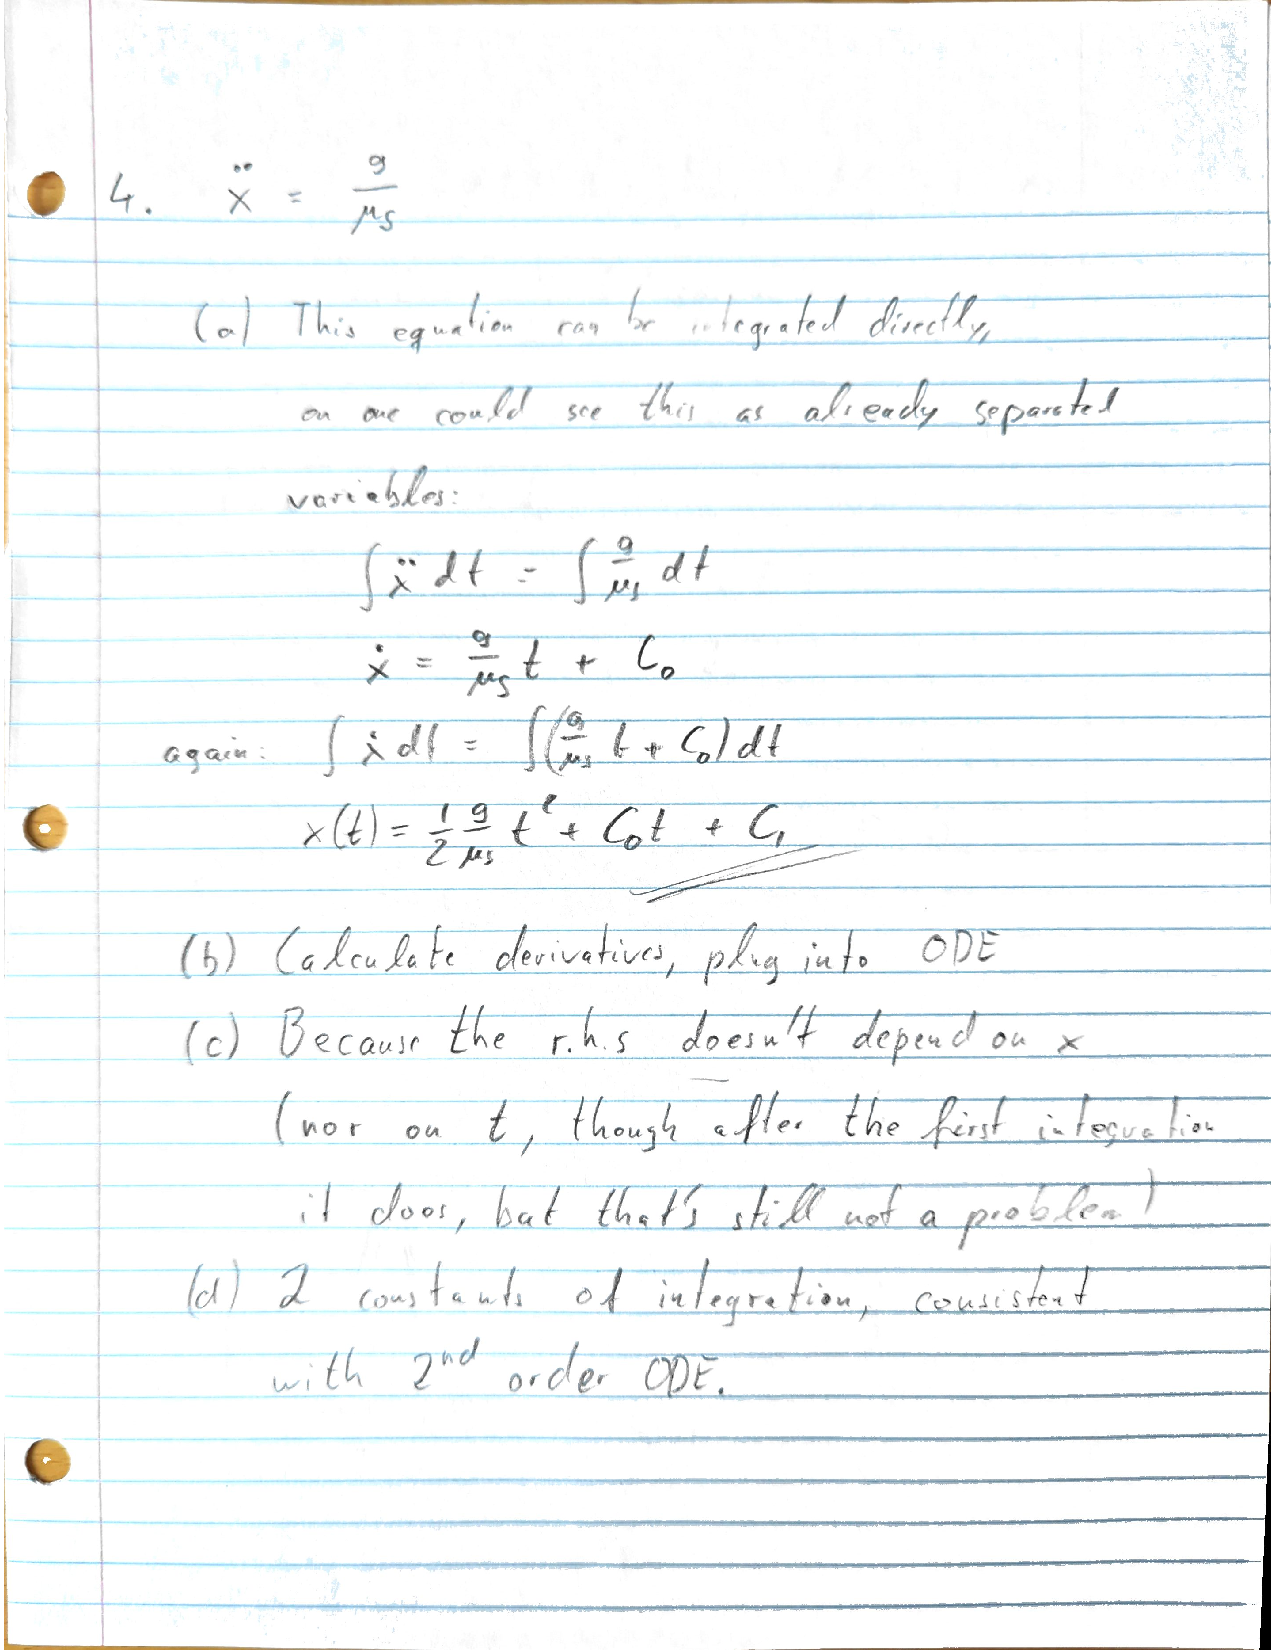
\includegraphics[page=1,width=\textwidth]{hw2-45.pdf}
  }

  \item TQQ, D (5 points) \textbf{Back to the skateboard problem}

  In class, we used the small angle approximation to derive the ODE
  \begin{align}
      \ddot \phi = -\omega_0^2 \phi
  \end{align}

  (where $\omega_0$ is some presumably known parameter, ie., the angular frequency). We used some educated guessing to find the general solution
  \begin{align}
      \phi(t) = A \cos\omega_0 t + B \sin\omega_0 t
  \end{align}

  \begin{enumerate}
  \item How would you go about verifying that this truly is a solution to the ODE above? (You don't have to do it, though it might not hurt to do so.)
  \item Find the angular velocity $\omega(t) = \dot \phi$, that is, how fast the skateboard is actually moving at a given point in time.

  Note that there is some possible confusion here, with all the $\omega$'s. $\omega_0$ is the (constant) angular frequency of the oscillation itself, so that's basically telling you how many times per second the skateboard is going back and forth. (A better way might be to think in terms of the regular frequency $f$, related by $\omega_0 = 2\pi f$.) On the other hand, the angular velocity tells you how fast the angle $\phi$ is changing at a given point in time. E.g., if you put the skateboard at $30^\circ$ and let go at time 0, at that very time, the angle is not changing yet, so angular velocity is still 0, but it's just about to increase (well, technically, it decreases since it goes to a negative value, as the angle starts to decrease towards 0, ie., the bottom of the halfpipe.)

  \item Let's say the skateboard is being held at an angle of $\phi_0$ (at rest), and then let go at time $t = 0$. Determine the constants $A$, $B$ in the general solution above.

  \soln{

  \includegraphics[page=2,width=\textwidth]{hw2-45.pdf}
  }

  \end{enumerate}


  % \item TQQ (10 points) Solve the separable differential equation
  % $$
  % \frac{dv}{dt} = a - bv
  % $$

  % where $a$ and $b$ are constants. Take the velocity at $t=0$ to be $v_0$.  Once you have that solution, find $y(t)$ given
  % $$\frac{dy}{dt} = v(t)$$

  % Be sure to plug in your functional form for $v(t)$ that you got from the first part of this problem.  Also, take $y(0)=y_0$.

  \clearpage
  \item	TQQ (4 points) Look at the following differential equations.  If they are separable, put them in the form that allows us to integrate them (but you do not need to do the integration).  If they are not separable, state that.  Take $t$ and $v$ to be our independent and dependent variables, $a$, $b$  are constants.
  \begin{enumerate}
    \item $$\frac{dv}{dt} = av^2 + t^3$$
    \item $$\frac{dv}{dt} = b + t^3$$
    \item $$\frac{dv}{dt} = \frac{1}{b + v^3}$$
    \item $$\frac{dv}{dt} = c\sqrt{vt}$$
  \end{enumerate}

  \soln{
    \begin{enumerate}
      \item not possible
      \item $$dv = (b + t^3) dt$$
      \item $$(b+v^3)dv = dt$$
      \item $$\frac{dv}{\sqrt{v}} = c\sqrt{t}dt$$
    \end{enumerate}

  }

\item BF (5 points) From the definition of Taylor series, derive the MacLaurin series (expanding around $t=0$) for $e^t$  and $e^{it}$ (where $i^2=-1$) out to the fourth order term.

\soln{
  \begin{align*}
  e^t &= e^0 + t\left.\frac{d(e^t)}{dt}\right|_0 +
  \frac{1}{2} t^2 \left.\frac{d^2(e^t)}{dt^2}\right|_0 +
  \frac{1}{3!} t^3\left.\frac{d^3(e^t)}{dt^3}\right|_0 +
  \frac{1}{4!} t^4\left.\frac{d^4(e^t)}{dt^4}\right|_0\\
  &= 1 + t + \frac{1}{2} t^2 + \frac{1}{6}t^3 + \frac{1}{24}t^4\\
  e^{it} &= e^0 + t\left.\frac{d(e^{it})}{dt}\right|_0 +
  \frac{1}{2} t^2 \left.\frac{d^2(e^{it})}{dt^2}\right|_0 +
  \frac{1}{3!} t^3\left.\frac{d^3(e^{it})}{dt^3}\right|_0 +
  \frac{1}{4!} t^4\left.\frac{d^4(e^{it})}{dt^4}\right|_0\\
  &= 1 + it - \frac{1}{2} t^2 - \frac{1}{6}it^3 + \frac{1}{24}t^4
  \end{align*}
}

\item TQQ (5 points)  The book derives $v(t)$ for an object falling and subject to linear drag.  The solution is (Eq 2.33)
$$v(t)=v_t \left(1-e^{-t/\tau} \right)$$
  where $\tau = m/b$ and $v_t = mg/b$.

  \begin{enumerate}\item
	Argue that in the case of linear drag, we would expect $v(t) \approx gt$ for short times.
  \item
	Use the Taylor expansion of the exponential function to verify that this solution meets that expectation.
	\item What do we mean by "short" times in this problem?  "Short" compared to what?  And how does the math set this time scale?
  \end{enumerate}

 \soln{
   \begin{enumerate}\item
      As the object starts from rest, its initial speed will be zero, and for some (short) time, it'll still be small (but growing). As long as its small, the drag force is small, and so we can neglect it and just have (almost) constant acceleration due to gravity, ie., $v(t) \approx gt$.

      \item The Taylor expansion gives $e^{-t/\tau} \approx 1 - \frac{t}{\tau}$. Plugging that in:
      \begin{align*}
        v(t) = v_t \left(1-e^{-t/\tau}\right) \approx v_t(1 - (1 - t/\tau)) = \frac{v_t}{\tau} t = gt
      \end{align*}

      \item $\tau$ sets the the time scale. We can see this by plugging in the expansion of $v(t) \approx v_t \frac{t}{\tau}$:
      \begin{align*}
        \dot v = \frac{1}{\tau}(-v + v_t) \approx \frac{1}{\tau}\left(-v_t \frac{t}{\tau} + v_t\right) = \frac{v_t}{\tau}\left(1 - \frac{t}{\tau}\right)
      \end{align*}
      Here we can see that acceleration is approximately constant if $t \ll \tau$ ie., $t/\tau \ll 1$.
   \end{enumerate}
 }

  \item 	BF, TQQ (10 points)  Introduction/Review of Hyperbolic functions.  These functions will arise several times this year as solutions to problems, so we will begin by becoming a bit more familiar with them. Beginning with the definitions of the hyperbolic functions:

  \begin{align*}
    \cosh x &=  \frac{e^x+e^{-x}}{2}\\
    \sinh x &=  \frac{e^x-e^{-x}}{2}\\
    \tanh x &=  \frac{\sinh x}{\cosh x}
  \end{align*}

  \begin{enumerate}\item
    Evaluate $e^x$, $e^{-x}$, $\sinh x$, $\cosh x$, $\tanh x$ at $x = -\infty, 0, \infty$.

    \soln{
      \begin{tabular}{llll}
        \hline\hline
        $f(x)$ & $f(\-\infty)$ & $f(0)$ & $f(\infty)$\\\hline
        $e^x$ & $0$ & $1$ & $\infty$\\
        $e^{-x}$ & $\infty$ & $1$ & $0$\\
        $\sinh x$ & $-\infty$ & $0$ & $\infty$\\
        $\cosh x$ & $\infty$ & $1$ & $\infty$\\
        $\tanh x$ & $-1$ & $0$ & $1$\\
        \hline\hline
      \end{tabular}
    }
    \item    Sketch $e^x$ and $e^{-x}$ for both positive and negative values of $x$.

    \soln{\\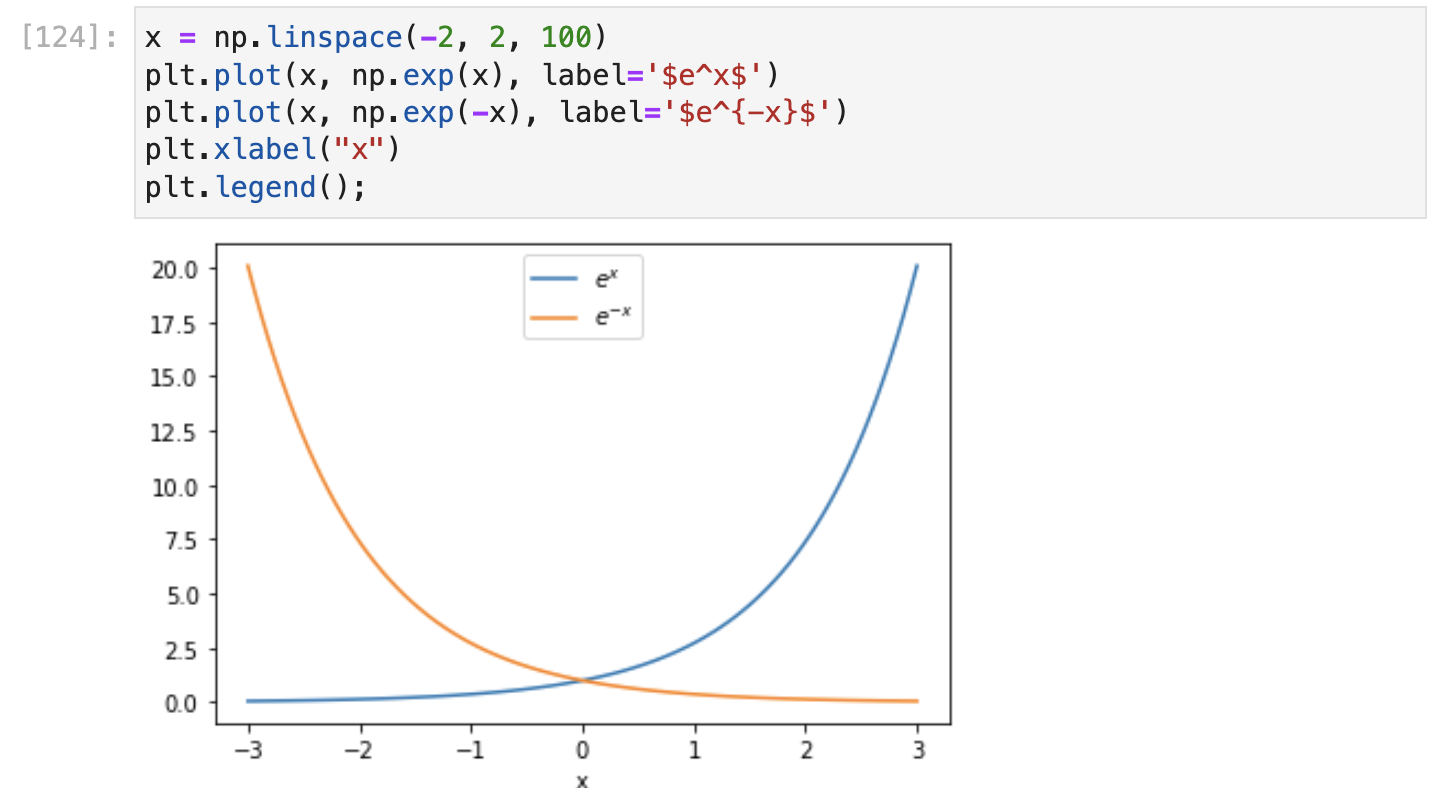
\includegraphics[width=.7\textwidth]{fig_exp.png}}

\item    Sketch $\cosh x$, $\sinh x$, $\tanh x$.

\soln{\\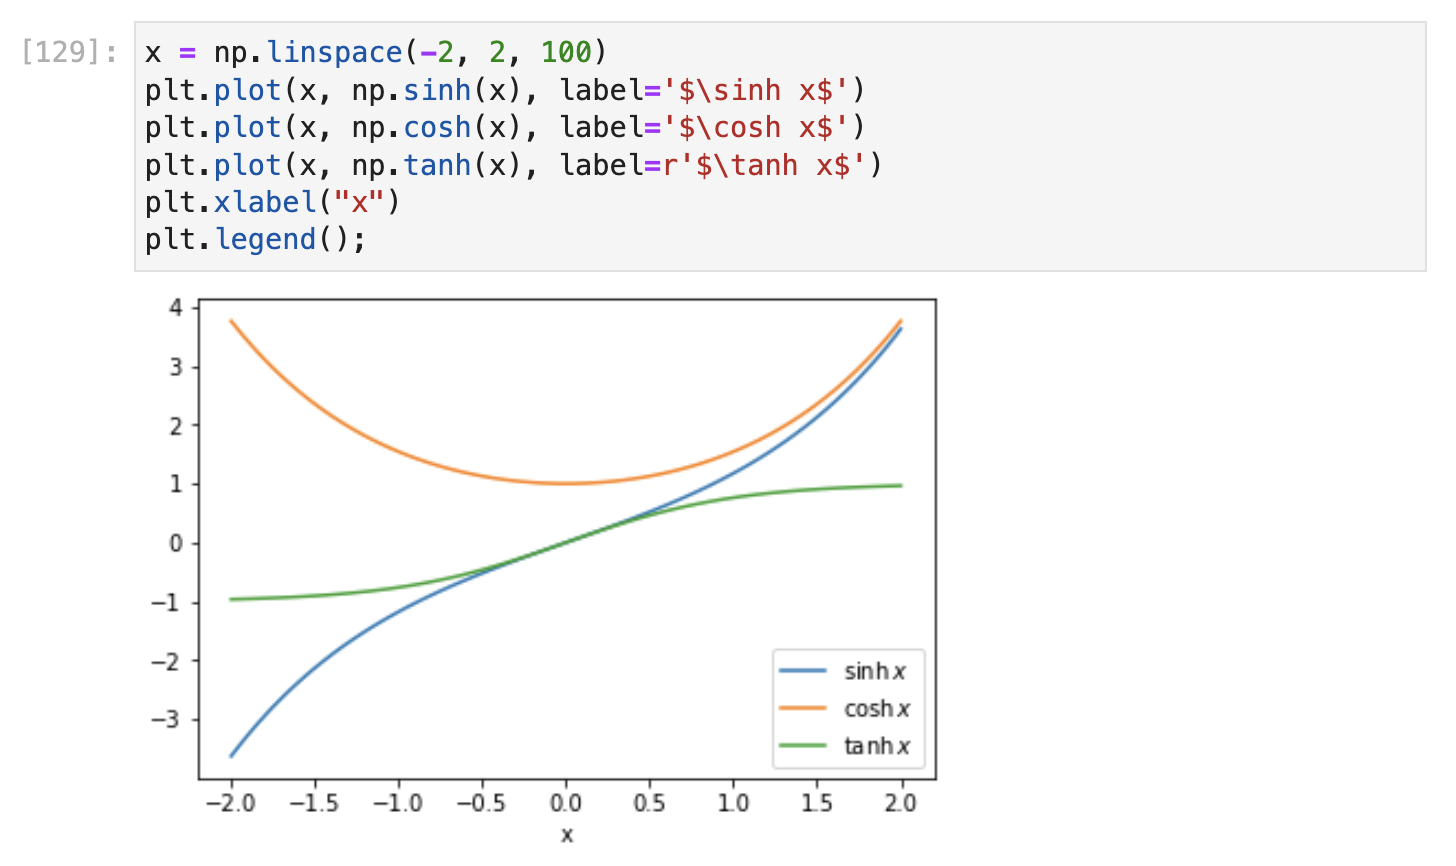
\includegraphics[width=.7\textwidth]{fig_hyp.png}}

\item    Show $\cosh^2 x - \sinh^2 x = 1$.

\soln{
  \begin{align*}
    \cosh^2 x - \sinh^2 x &= (\cosh x - \sinh x) (\cosh x + \sinh x)\\
    &= e^{-x}e^x \\
    &= 1
  \end{align*}
}

\item    Show that the derivative of the cosh is the sinh, and vice versa.

\soln{
  \begin{align*}
    \frac{d\cosh x}{dx} &= \frac{1}{2}\left(\frac{de^x}{dx} + \frac{de^{-x}}{dx}\right)\\
    &=\frac{1}{2}\left(e^x - e^{-x}\right) = \sinh x
  \end{align*}

and similarly for the derivative of sinh.
}

      \end{enumerate}

      \item	FC (10 points) (free choice): allows you to decide where to put your time.  Any of the following are possible: work through a section of the text or a lecture in detail; polish up a group work assignment from class; redo a problem from before; do an unassigned problem in the text; extend a computing project; try a problem using a different analytical approach (e.g. forces instead of conservation of energy).


\end{enumerate}

\end{document}
